% \documentclass[handout, xcolor=table]{beamer}
\documentclass[xcolor=table]{beamer}

\usepackage{fixcmex} % fix binomials

%-----------------------[ Macros ]----------------------------------------------%

%-----------------------[ Packages ]-------------------------------------------%

\usepackage[utf8]{inputenc}
% \usepackage[brazilian]{babel}
\usepackage[english]{babel}
\usepackage[T1]{fontenc}
\usepackage{lmodern}
\usepackage{amsfonts}
\usepackage{indentfirst}
\usepackage{xspace}
\usepackage{setspace}
\usepackage{geometry}
\usepackage{mathtools}
\usepackage{amsmath}
\usepackage{amsthm}
\usepackage{subcaption}
\usepackage{pdfpages}
\usepackage{hanging}
\usepackage{pdfpages}
\usepackage{nicefrac}
\usepackage{graphicx}
\usepackage[labelformat=empty]{caption}
\usepackage[shortlabels]{enumitem}
\usepackage{booktabs, multirow} % for borders and merged ranges
% \usepackage[hyperpageref]{backref}
% \usepackage[
%   scr=boondox, % heavily sloped
%   cal=esstix % slightly sloped
% ]{mathalpha}
\usepackage{xmpmulti}
\usepackage{appendixnumberbeamer}

% Tikz:
\usepackage{tikz}
% \usetikzlibrary{ipe} % ipe compatibility library
\usetikzlibrary{calc, arrows, arrows.meta, patterns}

\usepackage{macrossty}

%-----------------------[ Colors ]---------------------------------------------%

\definecolor{red}{rgb}{1,0,0}
\definecolor{blue}{rgb}{0,0,1}
\definecolor{green}{rgb}{0,1,0}
\definecolor{yellow}{rgb}{1,1,0}
\definecolor{orange}{rgb}{1,0.647,0}
\definecolor{gold}{rgb}{1,0.843,0}
\definecolor{purple}{rgb}{0.627,0.125,0.941}
\definecolor{gray}{rgb}{0.745,0.745,0.745}
\definecolor{brown}{rgb}{0.647,0.165,0.165}
\definecolor{navy}{rgb}{0,0,0.502}
\definecolor{pink}{rgb}{1,0.753,0.796}
\definecolor{seagreen}{rgb}{0.18,0.545,0.341}
\definecolor{turquoise}{rgb}{0.251,0.878,0.816}
\definecolor{violet}{rgb}{0.933,0.51,0.933}
\definecolor{darkblue}{rgb}{0,0,0.545}
\definecolor{darkcyan}{rgb}{0,0.545,0.545}
\definecolor{darkgray}{rgb}{0.663,0.663,0.663}
\definecolor{darkgreen}{rgb}{0,0.392,0}
\definecolor{darkmagenta}{rgb}{0.545,0,0.545}
\definecolor{darkorange}{rgb}{1,0.549,0}
\definecolor{darkred}{rgb}{0.545,0,0}
\definecolor{lightblue}{rgb}{0.678,0.847,0.902}
\definecolor{lightcyan}{rgb}{0.878,1,1}
\definecolor{lightgray}{rgb}{0.827,0.827,0.827}
\definecolor{lightgreen}{rgb}{0.565,0.933,0.565}
\definecolor{lightyellow}{rgb}{1,1,0.878}
\definecolor{black}{rgb}{0,0,0}
\definecolor{white}{rgb}{1,1,1}

%-----------------------[ Commands ]-------------------------------------------%

\newcommand\mycomment[1]{} % block comment

\newcommand{\dist}{\text{dist}}
\newcommand{\cost}{\text{cost}}
\newcommand{\opt}{\text{OPT}}
\newcommand{\makespan}{\emph{makespan}}

\newcommand{\cala}{\mathcal{A}}
\newcommand{\calb}{\mathcal{B}}
\newcommand{\calg}{\mathcal{G}}
\newcommand{\cali}{\mathcal{I}}
\newcommand{\call}{\mathcal{L}}
\newcommand{\calo}{\mathcal{O}}
\newcommand{\cals}{\mathcal{S}}
\newcommand{\calt}{\mathcal{T}}

\newcommand{\N}{\rm I\!N}
\newcommand{\overeps}{\nicefrac{1}{\varepsilon}}
\newcommand{\B}{$\bullet$}

\newcommand\rest[2]{\left.{#1}\right|_{#2}} % function restriction

\newcommand\set[1]{\{#1\}}

\DeclarePairedDelimiter\ceil{\lceil}{\rceil}
\DeclarePairedDelimiter\floor{\lfloor}{\rfloor}
\DeclareMathOperator*{\argmax}{arg\,max}
\DeclareMathOperator*{\argmin}{arg\,min}

\newcommand{\XSAT}{\textrm{XSAT}} % Exact SAT
\newcommand{\rXSAT}{$(2,1)$-\XSAT} % Exact SAT with 2 positive, 1 negative occurences of each variable
\newcommand{\rXthreeSAT}{\mbox{$1$-in-$3$-SAT$_{(2,1)}$}}%{$(2,1)$-X3SAT} % Exact SAT with 2 positive, 1 negative occurences of each variable, and clauses with size <= 3
\newcommand{\kXSAT}{$k$-\textrm{True} \rXSAT}
\newcommand{\kXthreeSAT}{$k$-\textrm{True} \rXthreeSAT}

%-----------------------[ Proof Environments ]---------------------------------%

% \newtheorem{definition}{Definição}
\newtheorem{thm}{Teorema}
\newtheorem{cor}{Corolário}
\newtheorem{conj}{Conjectura}
\newtheorem{lem}{Lema}
\newtheorem{obs}{Observação}
\newtheorem{remark}{Remark}
\newtheorem{proposition}{Proposition}

\newcounter{finalframe}
\newcommand{\stopcounter}{
  \setcounter{finalframe}{\insertframenumber}
}

\newcommand{\resumecounter}{
  \setcounter{framenumber}{\value{finalframe}}
}

\newcommand{\inccounter}{
  \setcounter{framenumber}{\value{finalframe} + 1}
}

%-----------------------[ Template ]-------------------------------------------%

\mode<presentation> {
    \usetheme[sectionpage=none, progressbar=frametitle, block=fill]{moloch} % modern fork of the metropolis theme
    \setbeamertemplate{footline}[frame number] % to replace the footer line in all slides with a simple slide count
}
\setbeamerfont{footnote}{size=\tiny}
\setbeamertemplate{navigation symbols}{}
\setbeamertemplate{footnote}{%
    \hangpara{2em}{1}%
    \makebox[2em][l]{\tiny\insertfootnotemark}%
    \hspace{-1em}\tiny\insertfootnotetext\par\vspace{0.2cm}%
}
\setbeamercolor{background canvas}{bg=white}

%-----------------------[ (Sub)Section Slides ]--------------------------------%

\AtBeginSection[]{
    \begin{frame}
    \vfill
    \centering
    \setbeamercolor{title}{bg=mDarkTeal,fg=black!2}
    \begin{beamercolorbox}[sep=8pt,center,shadow=true]{title}
        \usebeamerfont{title}\insertsectionhead\par%
    \end{beamercolorbox}
    \vfill
    \end{frame}
}

\makeatletter
\newcommand{\subseqslide}{
\begin{frame}
  \setbeamercolor{title}{bg=mDarkTeal,fg=black!2}
  \centering
  \begin{minipage}{22em}
    \raggedright
    \begin{beamercolorbox}[sep=8pt,center,shadow=true]{title}
        \usebeamerfont{title}\insertsectionhead\par%
    \end{beamercolorbox}
    \usebeamertemplate*{progress bar in section page}
    \par
    \ifx\insertsubsectionhead\@empty\else%
      \vskip-.6\baselineskip
      \usebeamercolor[fg]{subsection title}%
      \usebeamerfont{subsection title}%
      \insertsubsectionhead{}
    \fi
  \end{minipage}
  \par
  \vspace{\baselineskip}
\end{frame}
}

\AtBeginSubsection[]{%
\subseqslide

% \setcounter{tocdepth}{3}
% \frame<beamer>{ 
%   \frametitle{}
%   \centering
%   \begin{minipage}{20em}
%   \tableofcontents[
%     currentsection,currentsubsection,sectionstyle=show/hide,subsectionstyle=show/shaded/hide,subsubsectionstyle=show/show/hide/hide
%   ]    
%   \end{minipage}
% }
}
\makeatother

%-----------------------[ Title page ]-----------------------------------------%

\title{
Realizing Graphs with Cut Constraints\texorpdfstring
{\footnote{This work began during the 6th edition of the São Paulo Workshop on Optimization, Combinatorics, and Algorithms (WoPOCA). We thank the organizers and the agencies CNPq (process number 404315/2023-2) and FAEPEX (process number 2422/23).}{\hfill}}
}

\titlegraphic{
  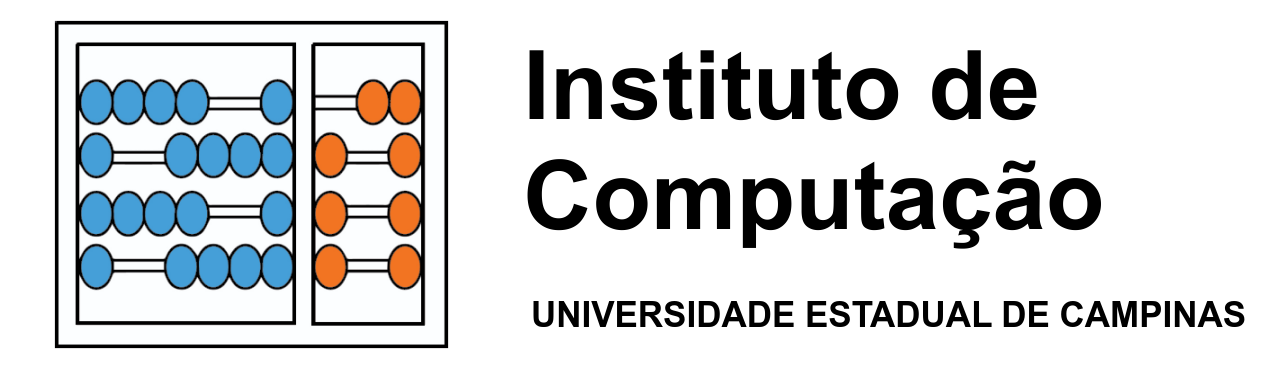
\includegraphics[height=1.cm]{logos/ic.png}
  \hfill
  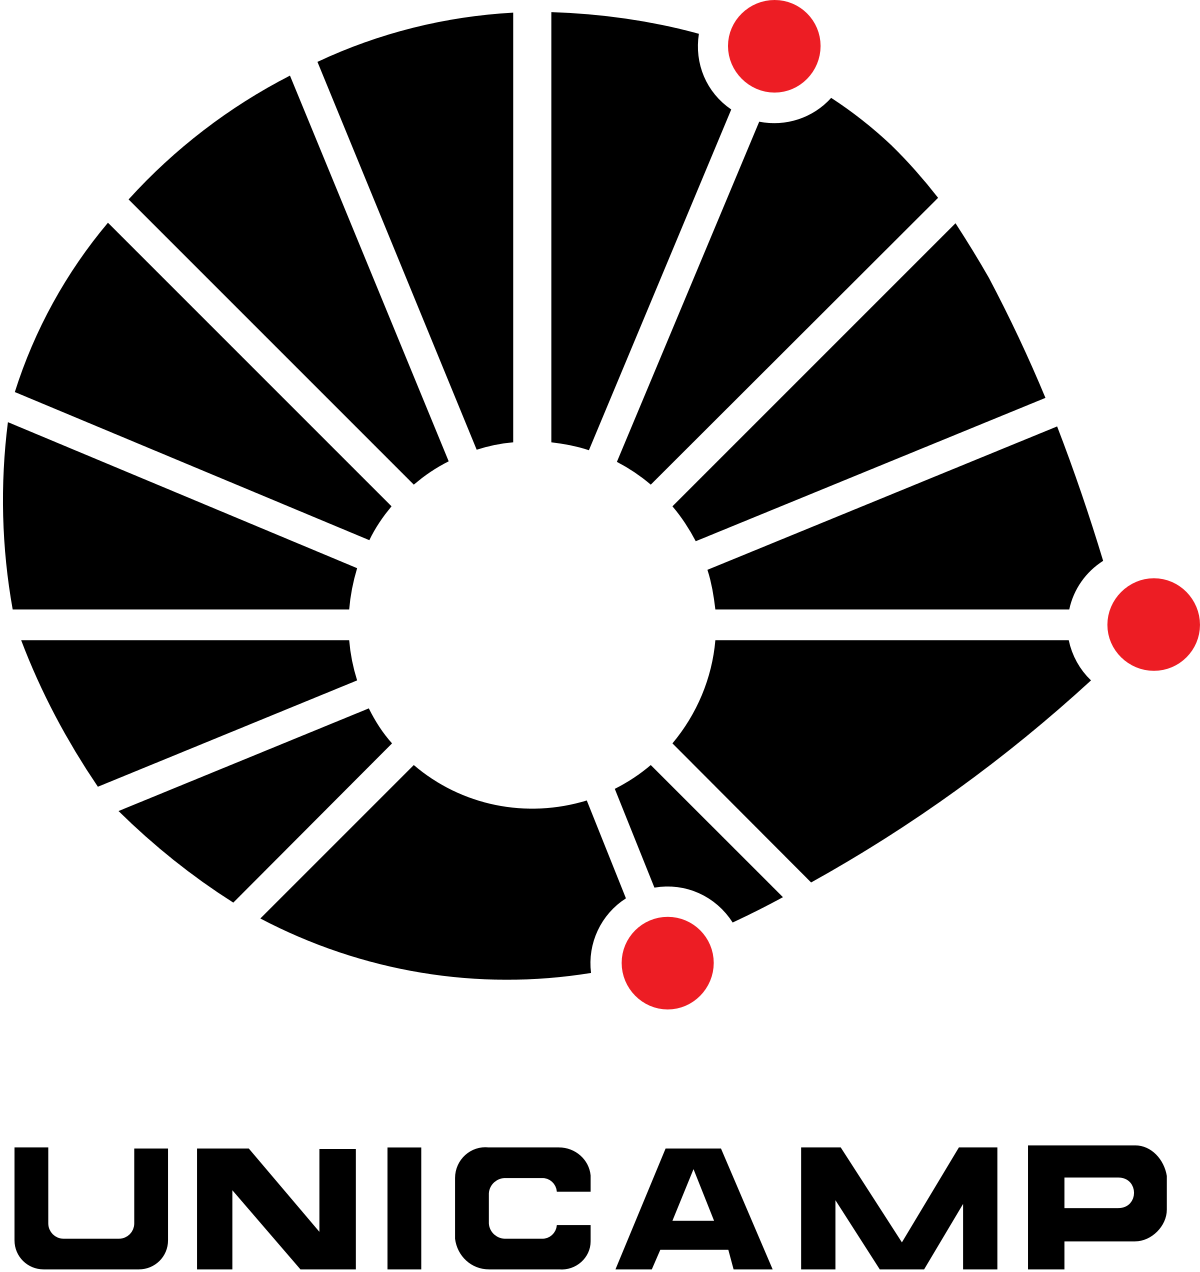
\includegraphics[height=1.2cm]{logos/unicamp.png}
}

\author{
\textbf{Lucas de Oliveira Silva}\inst{1}
\and \\
Vítor Gomes Chagas\inst{1}
\and \\
Samuel Plaça de Paula\inst{1}
\and \\
Greis Yvet Oropeza Quesquén\inst{1}
\and \\
Uéverton dos Santos Souza\inst{2,3}
}

\institute{
$^1$ Unicamp, Campinas, Brazil \newline
$^2$ IMPA, Rio de Janeiro, Brazil \newline
$^3$ UFF, Niterói, Brazil \\
}

\date{\vfill\hfill 14th CIAC, 11th June 2025}

\beamerdefaultoverlayspecification{<+->}

\begin{document}

\hyphenpenalty=10000

\begin{frame}[plain]
  \titlepage
\end{frame}

%------------------------------------------------------------------------------%

\section{Classic Problem}
\begin{frame}{Graph Realization Problem}
  \defproblema{Graph Realization}
    {A non-decreasing sequence $\texttt{d} = (d_1, \dots, d_n)$ of natural numbers.}
    {Is $\texttt{d}$ a graphic sequence?}
\end{frame}

\begin{frame}{Example}
  \centering
  Is $\texttt{d}=(3, 2, 2, 2, 1)$ graphic?
  \pause
  \bigbreak
  \begin{minipage}{\linewidth}
    \centering
    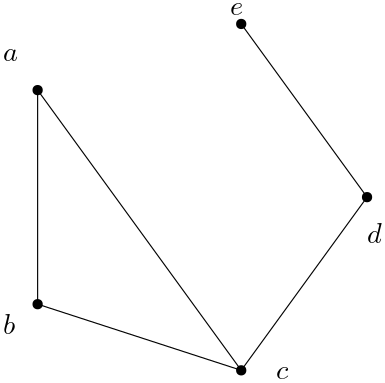
\includegraphics[height=4cm]{images/real1.png}
    \pause
    or
    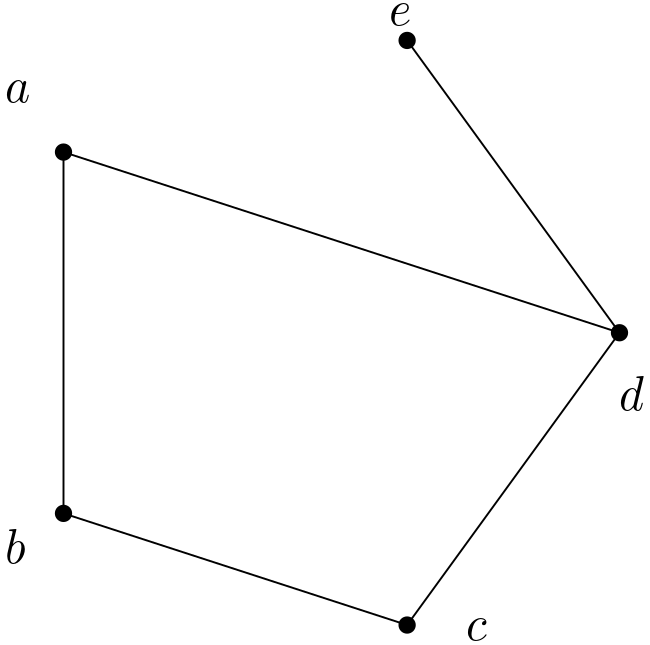
\includegraphics[height=4cm]{images/real2.png}
  \end{minipage}
\end{frame}

\begin{frame}{Graphic Sequences Characterization}
  \begin{theorem}[Erd\H{o}s and Gallai~\cite{erdos60}]
    A non-decreasing sequence $\texttt{d} = (d_1, \dots, d_n)$ of natural numbers is graphic if and only if \bigbreak
    
    1. $\sum\limits_{i=1}^n d_i$ is even, and \medskip

    2. For every $1 \le k \le n$,
        \[
        \sum_{i=1}^k d_i \le k(k - 1) + \sum_{i=k+1}^n \min\{d_i, k\}
        \]
  \end{theorem}
\end{frame}

\begin{frame}{Observations}
    \begin{enumerate}[-]
        \item Erd\H{o}s–Gallai gives a simple poly-time criterion;
        
        \item Many variations of the problem have been considered; 
        
        \item Vertex degree = size of trivial edge cut;
        
        \item We generalize this by adding nontrivial cut-size constraints.
    \end{enumerate}
\end{frame}

\begin{frame}{$k$-factors}
    \centering
    A \emph{$k$-factor} of a graph $G$ is a $k$-regular spanning subgraph of $G$.
    \bigbreak
    \pause
    A matching is a $1$-factor.
\end{frame}

\begin{frame}{$f$-factors}
    \centering
    A spanning subgraph $H$ of $G$ is a \emph{$f$-factor}, where $f \colon V \to \N$, if $d_H(v) = f(v)$ for all $v \in V$.
    \bigbreak
    \pause
    $f$-factors can be found in cubic time~\cite{Ans85}.
\end{frame}



\section{Nontrivial Cut Constraints}
\begin{frame}{Preliminaries}
    For a fixed graph $G = (V, E)$ where $V = \{v_1, \dots, v_n\}:$
    \pause
    \bigbreak
    \begin{enumerate}[-]
        \item A \emph{cut list} is a list of pairs $\call = \{(S_1, \ell_1), \dots, (S_m, \ell_m)\}$;
        
        \item For each $j$, we have $\emptyset \ne S_j \subsetneq V$ and $\ell_j \in \N$;
        
        \item $G$ \emph{realizes} $\mathcal{L}$ if $|\partial(S_j)|=\ell_j$ for every $(S_j, \ell_j) \in \mathcal{L}$;

        \item By $w(\call)$ we denote $\max\limits_j\ |S_j|$.
    \end{enumerate}
\end{frame}

\begin{frame}{New Graph Realization Problem}
  \defproblema{Graph Realization with Cut Constraints (GR-C)}
    {A cut list $\call$ for a set of vertices \mbox{$V = \{v_1, \dots, v_n\}$}, and a non-decreasing sequence $\texttt{d} = (d_1, \dots, d_n)$ of natural numbers.}
    {Does there exist a (labeled) simple graph \mbox{$G = (V, E)$} such that, for every $j$, $d(v_j) = d_j$ and $G$ realizes $\call$?}
\end{frame}

\begin{frame}{Example}
  \centering
  Consider $\texttt{d}=(d_1 = 3, d_2 = 2, d_3 = 2, d_4 = 2, d_5 = 1)$ and $\call = \{(\{v_2, v_3\}, 4), (\{v_1, v_2, v_5\}, 2)\}:$
  \pause
  \bigbreak
  \begin{minipage}{\linewidth}
    \centering
    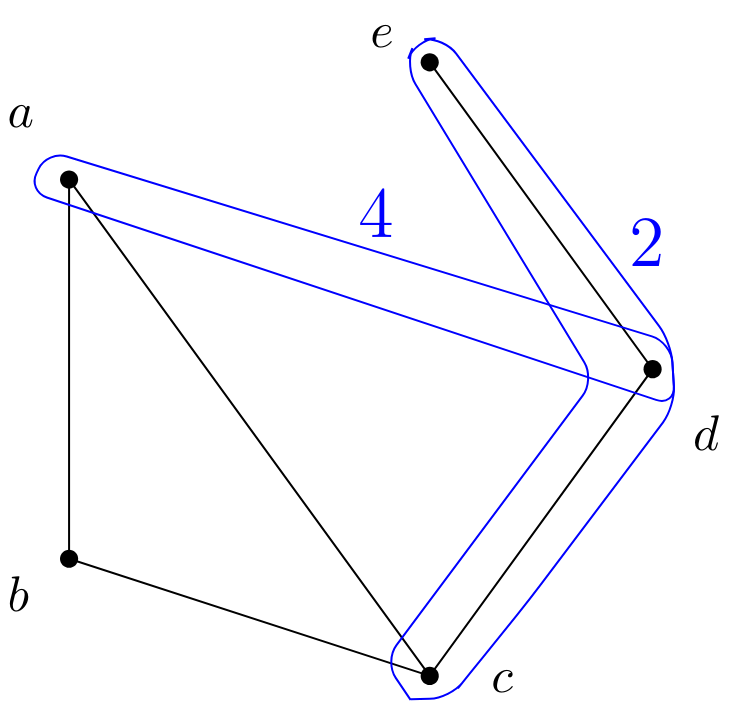
\includegraphics[height=4cm]{images/cut1.png}
  \end{minipage}
\end{frame}

\begin{frame}{Observations}
    \begin{enumerate}[-]

    \item If $\call = \emptyset$, we have GR;

    \item Assume that $2 \le |S_j| \le n-2$ for every $j$;

    \item If $\binom{V}{2} \subseteq \{S_j \mid (S_j, \ell_j) \in \mathcal{L}\} $ then the problem becomes trivial;

    \item GR-C can be seen as a consistency check for cut-queries.

  \end{enumerate}
\end{frame}

\begin{frame}{Important Remark}
    \centering
    For $S \subseteq V$ let $d(S) = \sum\limits_{v_j \in S} d_j$.
    \bigbreak
    \pause
    \begin{remark}[1]
        An instance $(\texttt{d}, \call)$ is true only if, for each $(S, \ell) \in \call$,
        \pause
        $\ell \in \{ d(S) - 2k \mid 0 \leq k \leq \binom{|S|}{2} \}$.
    \end{remark}
\end{frame}

\subsection{Small Cuts}

\begin{frame}{Fixed Edges}
    \centering
    If $(\set{u, v}, d_u + d_v - 2) \in \call$ then $uv \in E(G)$.
\end{frame}

\begin{frame}{Forbidden Edges}
    \centering
    If $(\set{u, v}, d_u + d_v) \in \call$ then $uv \notin E(G)$.
\end{frame}

\begin{frame}{A Single Case}
    \centering
    Replace $(\set{u, v}, d_u + d_v - 2)$ by $(\set{u, v}, d_u + d_v)$ while updating $\texttt{d}$.
\end{frame}

\begin{frame}{Possibility Graph}
    \centering
    Let $F$ be the set of forbidden edges.
    \pause
    \bigbreak
    Then we call $\calg = K_n - F$ the \emph{possibility graph}.
\end{frame}

\begin{frame}{Size 2 Cut Constraints}
    \centering
    We can reduce GR-C to $f$-factor!
    \pause
    \bigbreak
    \begin{lemma}[1]
        An instance $(\texttt{d}, \call)$ of GR-C can be solved in polynomial time whenever $w(\call) = 2$.
    \end{lemma}
\end{frame}

\begin{frame}{Size 3 Cut Constraints}
    \centering
    We can reduce to the previous case!
    \pause
    \bigbreak
    \begin{theorem}[2]
        An instance $(\texttt{d}, \call)$ of GR-C can be solved in polynomial time whenever $w(\call) = 3$.
    \end{theorem}
\end{frame}

\begin{frame}{Proof Sketch}
    \centering
    Consider a cut $(S, \ell) \in \call$ where $S = \set{u, v, w}$.
    \pause
    \bigbreak
    As an example, let $d_u = d_v = d_w = 2$ (so $d(S) = 6$).
\end{frame}

\begin{frame}{Case $\ell = d(S) = 6$}
    \centering
    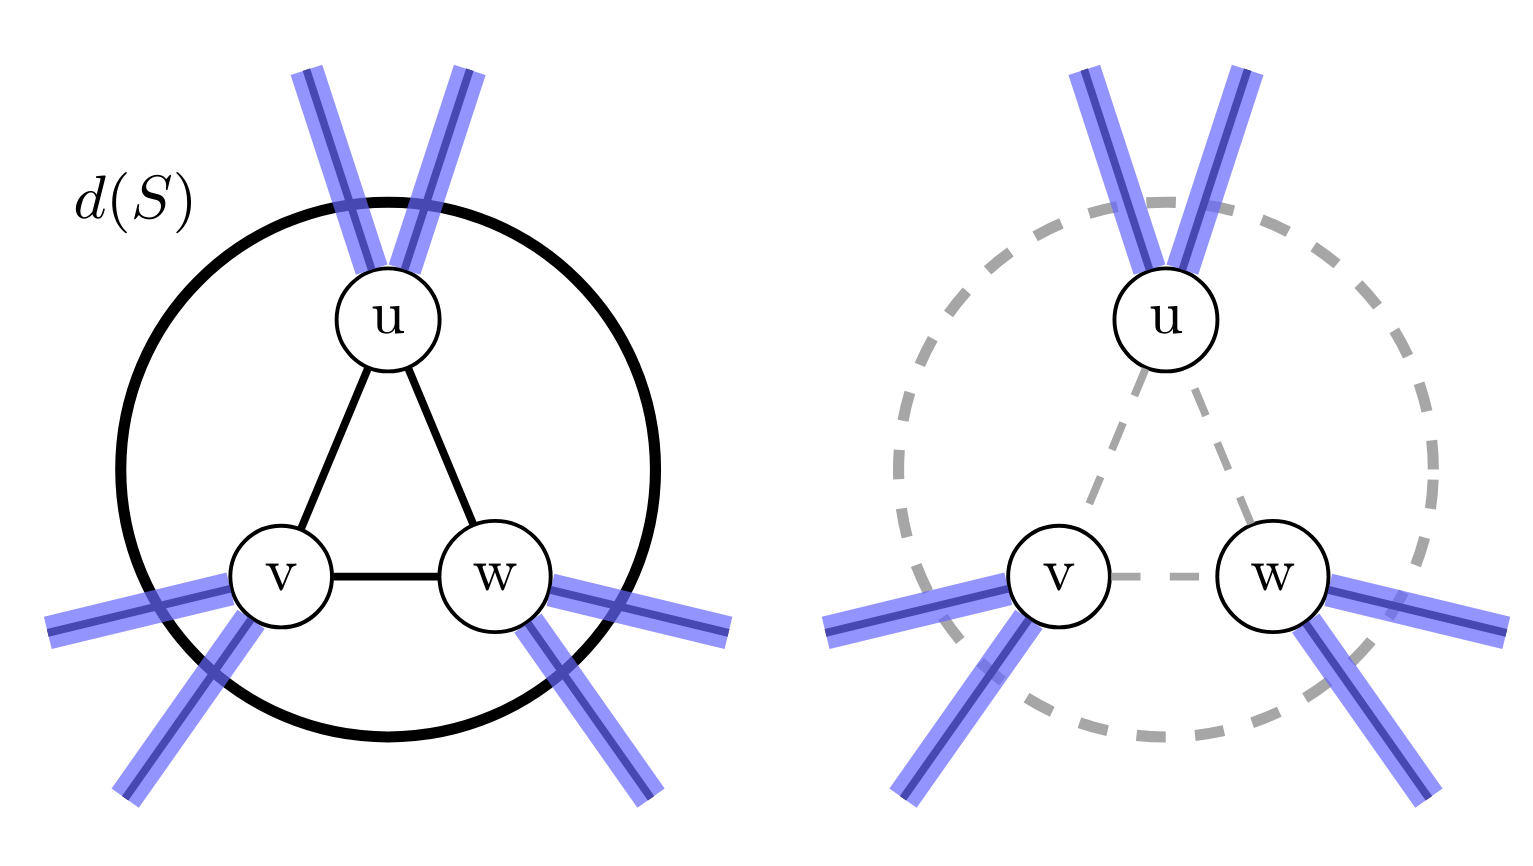
\includegraphics[height=4cm]{images/3cut1.png}
\end{frame}

\begin{frame}{Case $\ell = d(S) - 4 = 2$}
    \centering
    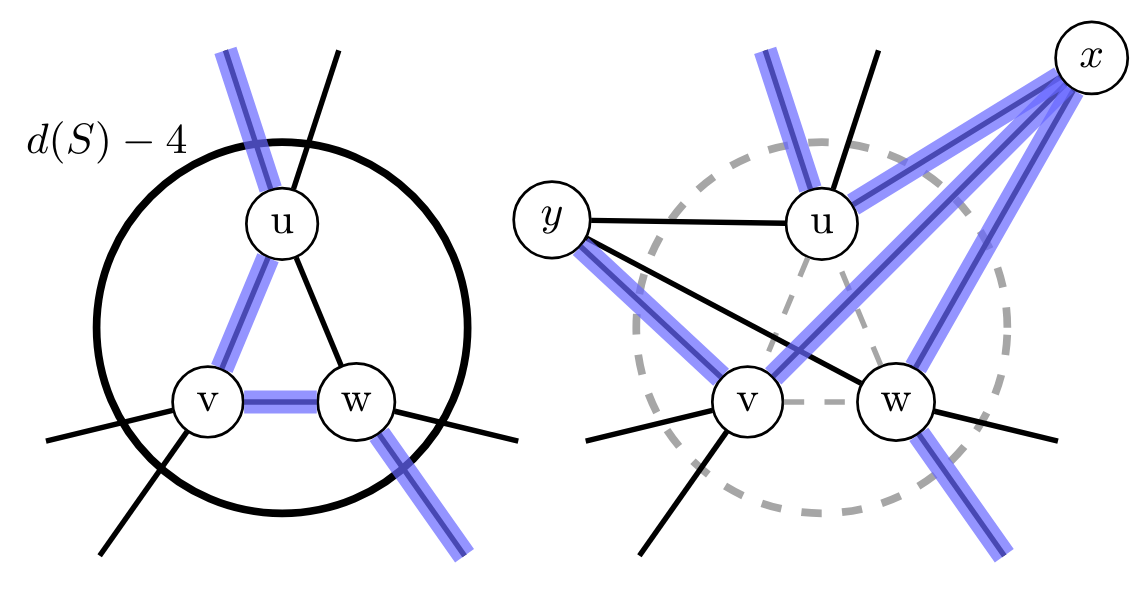
\includegraphics[height=4cm]{images/3cut4.png}
\end{frame}

\begin{frame}{Other Cases}
    \centering
    \Large
    \begin{align}
                    & \ell = d(S) - 2 = 4 \nonumber \\    
        \text{and } & \ell = d(S) - 6 = 0 \nonumber
    \end{align}
\end{frame}

\begin{frame}{Running Example}
  \centering
  $\texttt{d}=(d_1 = 3, d_2 = 2, d_3 = 2, d_4 = 2, d_5 = 1)$ and $\call = \{(\{v_2, v_3\}, 4), (\{v_1, v_2, v_5\}, 2)\}$:
  \bigbreak
  \begin{minipage}{\linewidth}
    \centering
    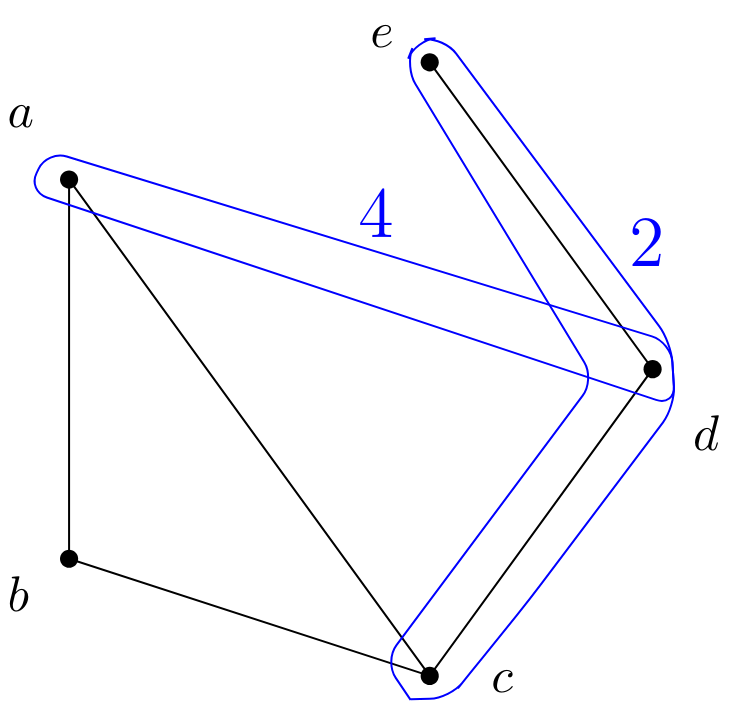
\includegraphics[height=6cm]{images/cut1.png}
  \end{minipage}
\end{frame}

\begin{frame}{Running Example}
  \centering
  Equivalent $f$-factor instance:
  \bigbreak
  \begin{minipage}{\linewidth}
    \centering
    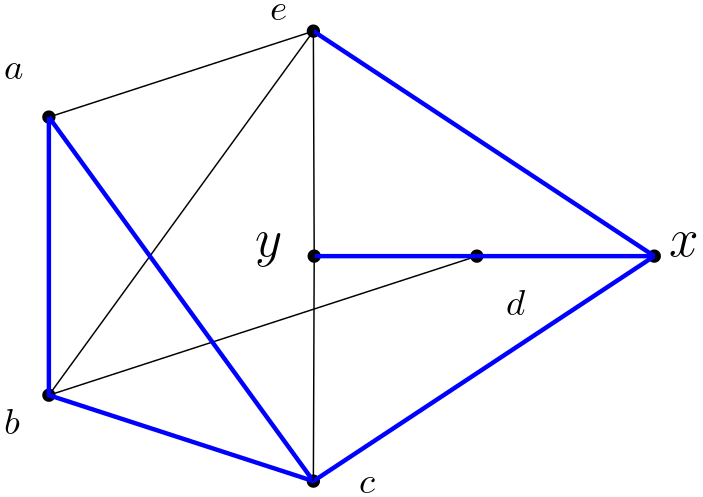
\includegraphics[height=4cm]{images/factor1.png}
  \end{minipage}
\end{frame}

\subsection{Large Cuts}

\begin{frame}{Size 4 Cut Constraints}
    \centering
    \Large
    Can we keep doing a case-by-case analysis?
    \pause
    \bigbreak
    No, we cannot, and the GR-C becomes hard!
\end{frame}

\begin{frame}{Intuition}
    \centering
    \Large
    For $S \in \binom{V}{3}$, $E[S]$ determines how degrees change.
    \pause
    \bigbreak
    In contrast, for $S \in \binom{V}{4}$, this claim no longer holds.
\end{frame}

\begin{frame}{Hardness}
    \centering
    \begin{theorem}[3]
        The GR-C problem cannot be solved in polynomial time unless $P = NP$ even when $w(\call) = 4$ and all degrees in the degree sequence $\texttt{d}$ are 1.
    \end{theorem}
\end{frame}

\begin{frame}{Proof}
    \centering
    \Large
    Reduction from $k$-True \rXthreeSAT{}
\end{frame}

\begin{frame}{\rXthreeSAT{}}
    \beamerdefaultoverlayspecification{}
    \defproblema{\rXthreeSAT{}}{
        A set of variables $X$ and a formula~$\phi$ in conjunctive normal form over $X$ such that:
        \begin{itemize}
            \item each variable of $X$ occurs twice as a positive literal and once as a negative literal;
            \item each clause of $\phi$ has two or three literals.
        \end{itemize}
    }{Is there a truth assignment of $X$ such that exactly one literal in every clause of $\phi$ is true?}
\end{frame}

\begin{frame}{\rXthreeSAT{}}
    \begin{lemma}[2]
        \rXthreeSAT{} is NP-complete.
    \end{lemma}
\end{frame}

\begin{frame}{\kXthreeSAT{}}
    \defproblema{\kXthreeSAT{}}{
        A tuple $(X, \phi, k)$, where $(X, \phi)$ is an instance of \rXthreeSAT{} and $k$ is a nonnegative integer.
    }{Is there a feasible solution to $(X, \phi)$ in which exactly $k$ variables are assigned to true?}
\end{frame}

\begin{frame}{\kXthreeSAT{}}
    \begin{lemma}[3]
        \kXthreeSAT{} cannot be solved in polynomial time unless $P = NP$.
    \end{lemma}
\end{frame}

\begin{frame}{Variable Gadget}
    \begin{minipage}{\linewidth}
        \centering
        \only<1>{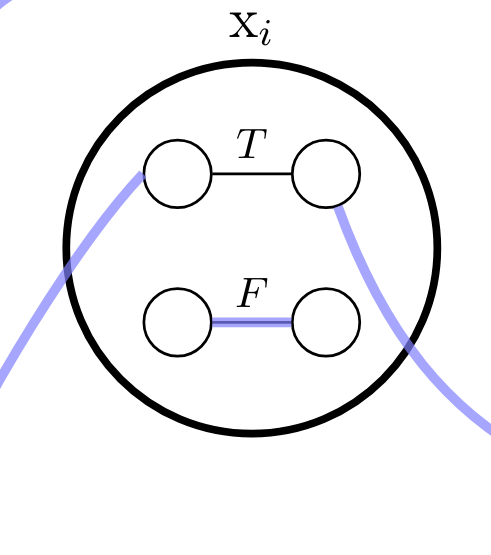
\includegraphics[clip, trim={0 0 0 0.2cm}, height=4.7cm]{images/reduction/true.png}}
        \only<2>{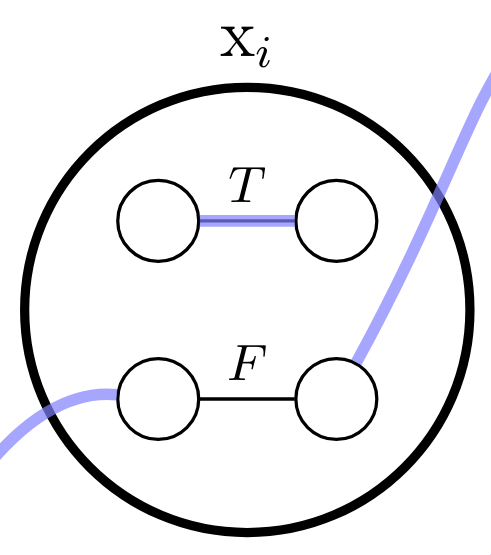
\includegraphics[height=4cm]{images/reduction/false.png}}
    \end{minipage}
\end{frame}

\begin{frame}{Clause Gadget}
    \centering
    $C_j = (x_a + x_b + x_c)$ and $C_k = (x_d + \bar x_e)$
    \bigbreak
    \begin{minipage}{\linewidth}
        \centering
        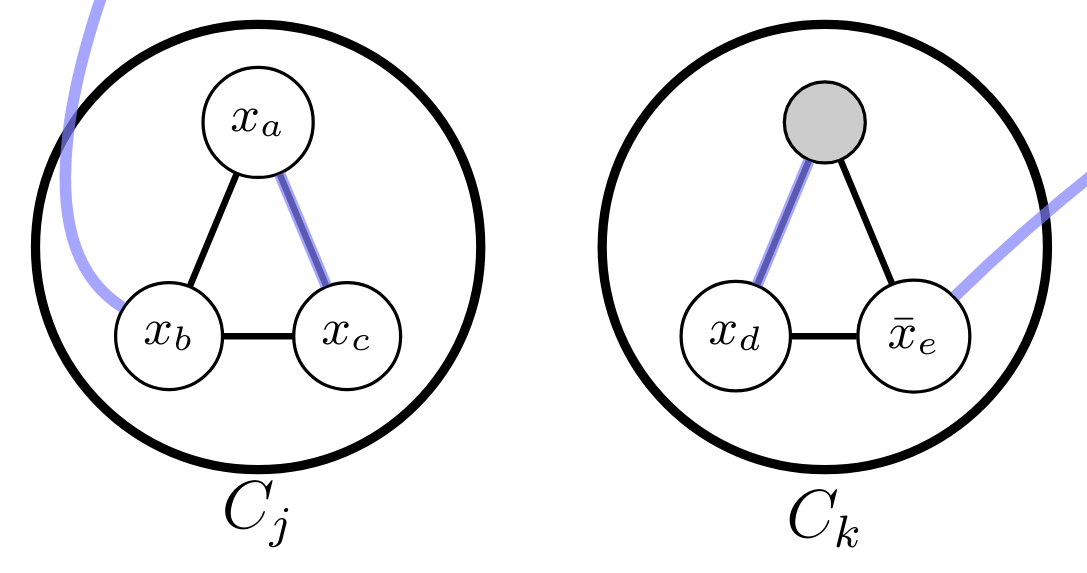
\includegraphics[height=4cm]{images/reduction/clause.png}
    \end{minipage}
\end{frame}

\begin{frame}{Complete Example}
    \centering
    $(\bar{x}_1 + x_3)(x_1 + x_2 + x_4)(x_1 + \bar{x}_4)(\bar{x}_2 + \bar{x}_3)(x_2 + x_3 + x_4)$ and $k=1$:
    \begin{figure}
        \centering
        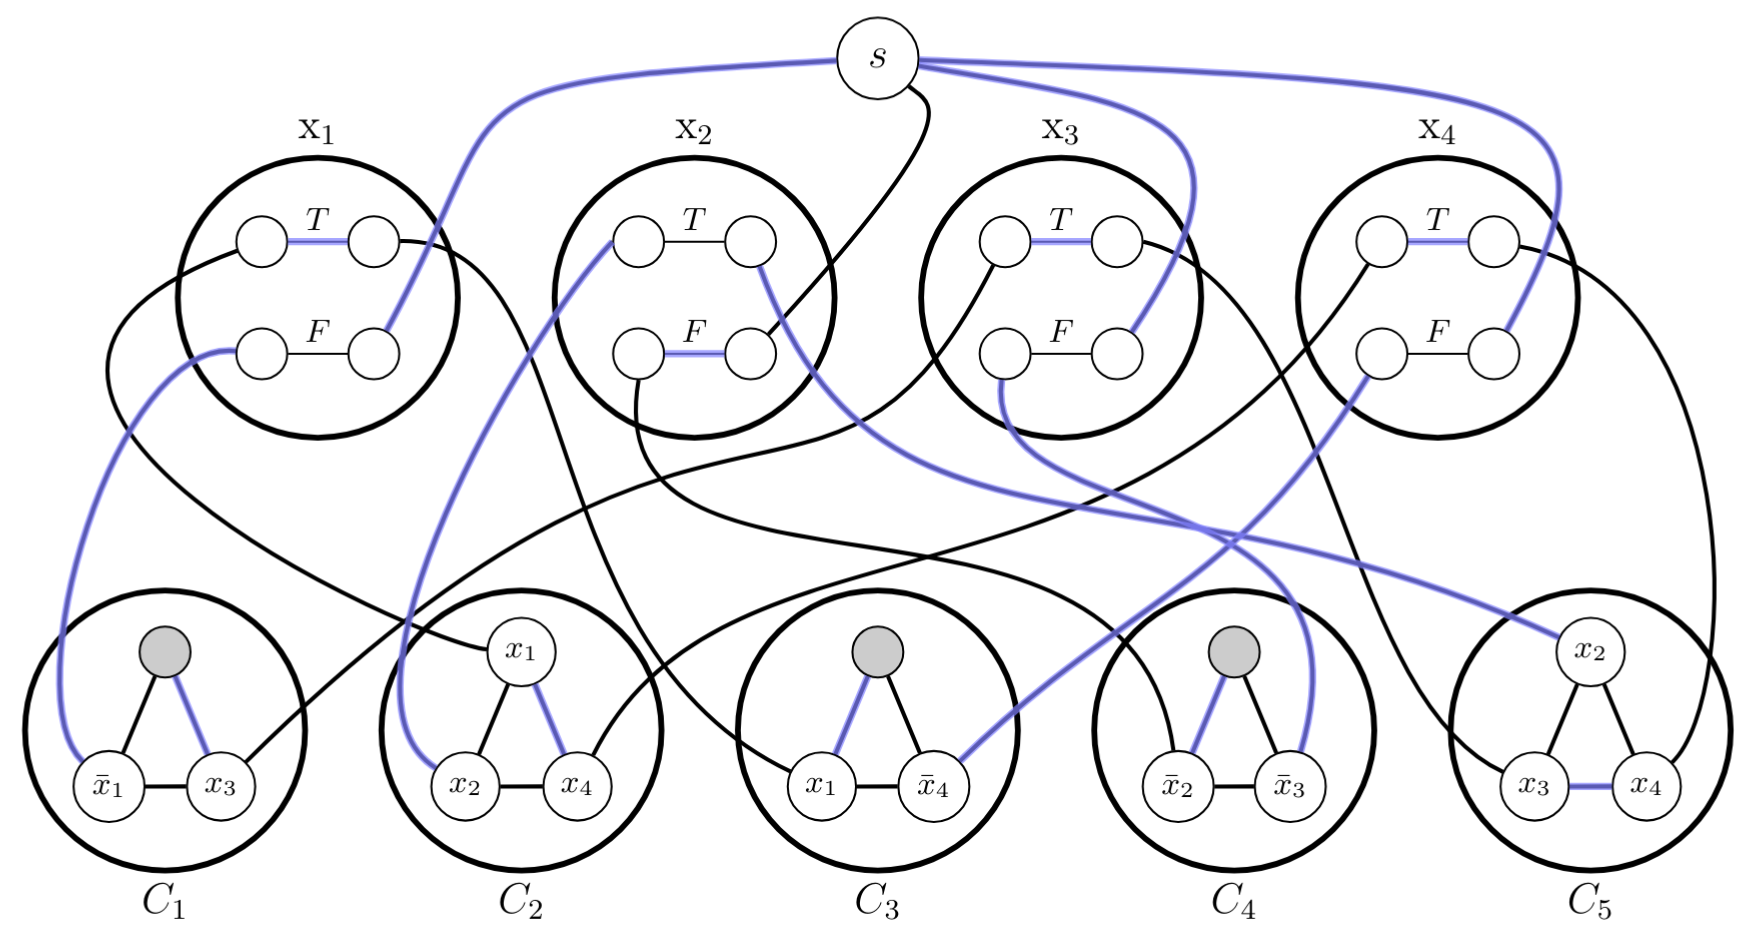
\includegraphics[width=0.9\textwidth]{images/reduction/full.png}
    \end{figure}
\end{frame}


\section{Conclusion}
\begin{frame}{Tree Possibility Graph}
    \begin{proposition}[1]
        Given an instance $(\texttt{d}, \call)$ of GR-C with a tree possibility graph $\calg$, we can decide if there is a solution in polynomial time.
    \end{proposition}
\end{frame}

\begin{frame}{Bipartite Possibility Graph}
    \begin{theorem}[3]
        The GR-C problem is NP-complete when the possibility graph $\calg$ is subcubic and bipartite, even when $w(\call) = 6$ and \texttt{d} is a sequence of ones.
    \end{theorem}
\end{frame}

\begin{frame}{Open Problems}
    \centering
    \only<1>{$\calg$ is planar or has bounded treewidth}
    \only<2>{The size of $\call$ is small (like $|\call|=1$)}
    \only<3>{Complexity of {1-in-3 SAT}$_{(2,2)}$}
    \only<4>{Geometric version of GR-C \vfill}
    \only<4>{
        \begin{minipage}{\linewidth}
            \centering
            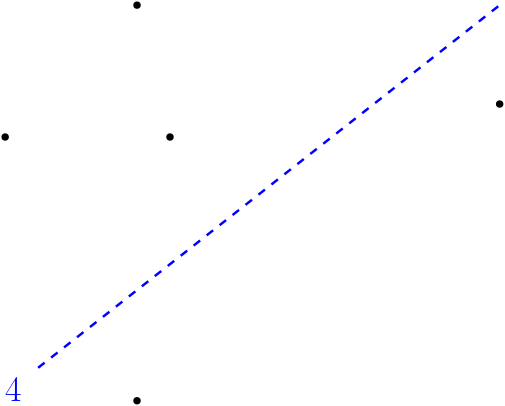
\includegraphics[height=4cm]{images/geom1.png}
        \end{minipage}
    }

    \only<5>{Polygon Realization with Cut Constraints \vfill}
    \only<5>{
        \begin{minipage}{\linewidth}
            \centering
            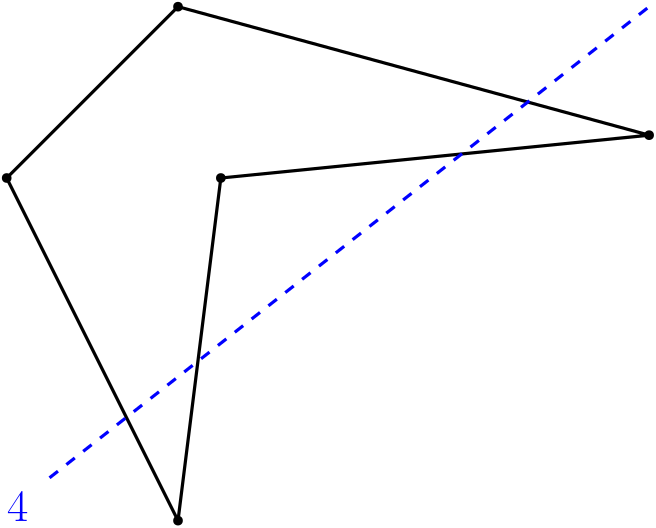
\includegraphics[height=4cm]{images/geom2.png}
        \end{minipage}
    }
\end{frame}

\begin{frame}
  \large{\centerline{Thank you all for the attention...}}
  \Huge{\centerline{The End}}
\end{frame}

%-----------------------[ Bibliography ]---------------------------------------%

\appendix

\beamerdefaultoverlayspecification{}
\setbeamertemplate{bibliography item}[text]
\begin{frame}
  \frametitle{Bibliography}
  {
    \tiny
    \bibliographystyle{alpha}
    \bibliography{bibliography}
  }
\end{frame}

%-----------------------[ Backup ]---------------------------------------------%


\end{document}
